\documentclass[../../Problems]{subfiles}
\begin{document}
\KOMAoptions{paper=A3}
\recalctypearea
\subsection{Quicksort}
Quicksort is a divide and conquer algorithm like merge sort discused in class. It first divides the input array into two smaller sub-arrays: the low elements and the high elements. It then
recursively sorts the sub-arrays. Precisely,
\begin{itemize}
	\item Pick an element, called a pivot, from the array.
	\item Reorder the array so that all elements with values less than the pivot come before the pivot, while all elements with values greater than the pivot come after it (equal values can go either way). After this \emph{partitioning}, the pivot is in its final position (relative to other elements).
	\item Recursively apply the above steps to the sub-array of elements with smaller values and separately to the sub-array of elements with greater values. The base case of the recursion are arrays of size zero or one, which are in order by definition, so they never need to be sorted.
\end{itemize}
\begin{note}
	The pivot selection and partitioning steps can be done in several different ways; the algorithm's performance greatly varies with implementation schemes.
\end{note}
\begin{figure}[H]
	\centering
	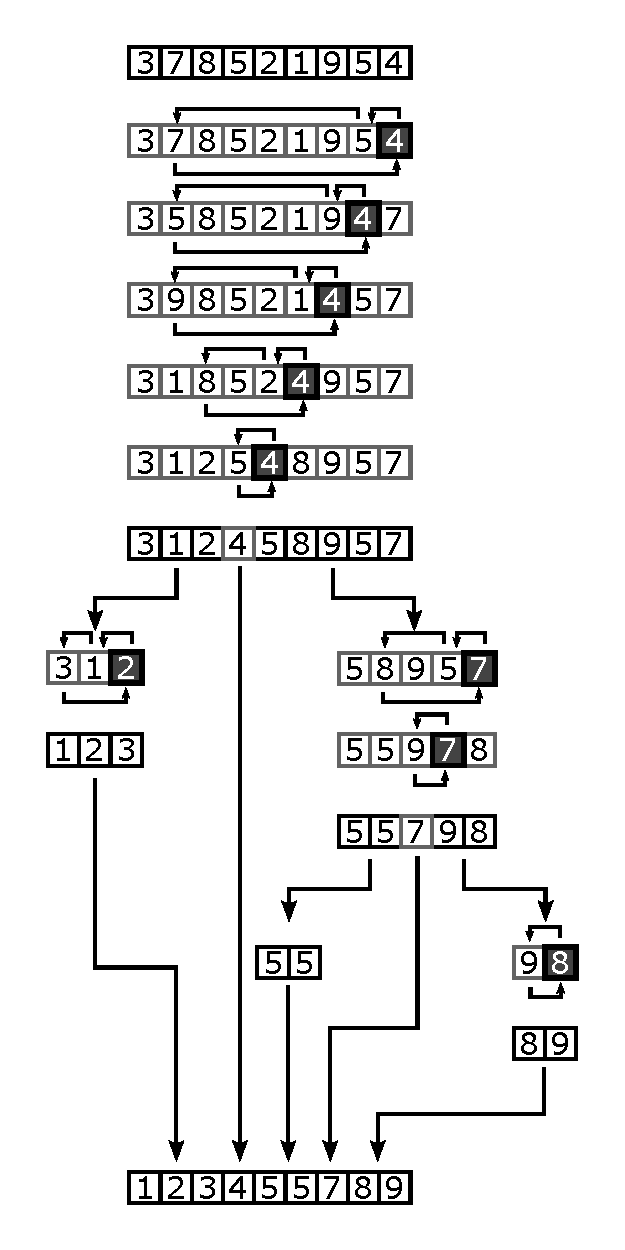
\includegraphics[width = 0.3\linewidth]{QuickSort.pdf}
	\caption{Quicksort Runthrough (\href{https://commons.wikimedia.org/wiki/File:Quicksort-diagram.svg}{Image} by \href{https://commons.wikimedia.org/wiki/User:Znupi}{Znupi}, Public domain, via Wikimedia Commons)}
	\label{fig:quicksort}
\end{figure}
\textbf{Problem Statement:}\\
Sort the given array using Quicksort. Use Lomuto partition scheme, i.e. take the last element of array as pivot.
\begin{note}
	You are not provided with the size of array. Learn the way to do it! If you give up then go through procedure in starter code and understand it thoroughly.
\end{note}
\begin{testcases}
	{$t$ \hfill(number of test cases, an integer)\\
	$a_0\ a_1\ a_2 \cdots a_{n_i-1}$ \hfill($n_i$ space seperated integers for each testcase)}
	{Sorted Array\hfill(space seperated elements for each test case)}
	{$1\leq n_i \leq 1000, -100000\leq a_{i}\leq 100000$\hfill(integers)}
	{4\\
	1 7 5 2 3 10 4 6 9 8\\
	86 56 24 26 55 73 77 100 53 20 52 59 74 43 19 21 74 51 44 79 76 15 54 62 6 43 42 5 28 84\\
	17 9 10 6 6 12 5 16 18 1 14 11 6 12 14 12 13 10 12 3 2 16 16 14 11 12 7\\
	59 18 -85 99 87 -90 -17 -83 -28 -19 -39 46 -27 -20 53 48 -11 -42 5 85 -49 78 86 -42 -33 -56 -41 21 -62 95 -59 -63 50 57 78 -8 14 -35 -5 7 4 -45 -17 -10 -23}
	{1 2 3 4 5 6 7 8 9 10\\
	5 6 15 19 20 21 24 26 28 42 43 43 44 51 52 53 54 55 56 59 62 73 74 74 76 77 79 84 86 100\\
	1 2 3 5 6 6 6 7 9 10 10 11 11 12 12 12 12 12 13 14 14 14 16 16 16 17 18\\
	-90 -85 -83 -63 -62 -59 -56 -49 -45 -42 -42 -41 -39 -35 -33 -28 -27 -23 -20 -19 -17 -17 -11 -10 -8 -5 4 5 7 14 18 21 46 48 50 53 57 59 78 78 85 86 87 95 99}
	{https://github.com/paramrathour/CS-101/tree/main/Starter Codes/Quicksort.cpp}
\end{testcases}
\begin{funvideo}
	\href{https://youtu.be/WaNLJf8xzC4}{What's the fastest way to alphabetize your bookshelf? - Chand John -- TED-Ed}
\end{funvideo}
\KOMAoptions{paper=A4}
\recalctypearea
\end{document}